\documentclass[12pt,letterpaper]{article}
\usepackage{graphicx,textcomp}
\usepackage{natbib}
\usepackage{setspace}
\usepackage{fullpage}
\usepackage{color}
\usepackage[reqno]{amsmath}
\usepackage{amsthm}
\usepackage{fancyvrb}
\usepackage{amssymb,enumerate}
\usepackage[all]{xy}
\usepackage{endnotes}
\usepackage{lscape}
\newtheorem{com}{Comment}
\usepackage{float}
\usepackage{hyperref}
\newtheorem{lem} {Lemma}
\newtheorem{prop}{Proposition}
\newtheorem{thm}{Theorem}
\newtheorem{defn}{Definition}
\newtheorem{cor}{Corollary}
\newtheorem{obs}{Observation}
\usepackage[compact]{titlesec}
\usepackage{dcolumn}
\usepackage{tikz}
\usetikzlibrary{arrows}
\usepackage{multirow}
\usepackage{xcolor}
\newcolumntype{.}{D{.}{.}{-1}}
\newcolumntype{d}[1]{D{.}{.}{#1}}
\definecolor{light-gray}{gray}{0.65}
\usepackage{url}
\usepackage{listings}
\usepackage{color}

\definecolor{codegreen}{rgb}{0,0.6,0}
\definecolor{codegray}{rgb}{0.5,0.5,0.5}
\definecolor{codepurple}{rgb}{0.58,0,0.82}
\definecolor{backcolour}{rgb}{0.95,0.95,0.92}

\lstdefinestyle{mystyle}{
	backgroundcolor=\color{backcolour},   
	commentstyle=\color{codegreen},
	keywordstyle=\color{magenta},
	numberstyle=\tiny\color{codegray},
	stringstyle=\color{codepurple},
	basicstyle=\footnotesize,
	breakatwhitespace=false,         
	breaklines=true,                 
	captionpos=b,                    
	keepspaces=true,                 
	numbers=left,                    
	numbersep=5pt,                  
	showspaces=false,                
	showstringspaces=false,
	showtabs=false,                  
	tabsize=2
}
\lstset{style=mystyle}
\newcommand{\Sref}[1]{Section~\ref{#1}}
\newtheorem{hyp}{Hypothesis}

\title{Problem Set 3}
\date{Due: November 20, 2022}
\author{Applied Stats/Quant Methods 1}


\begin{document}
	\maketitle
	
	
	\section*{Question 1}
	\vspace{.1cm}
	
	\begin{enumerate}
		\item \textbf{Run a regression where the outcome variable is \texttt{voteshare} and the explanatory variable is \texttt{difflog}.}	\vspace{.5cm}
		
		\lstinputlisting[language=R, firstline=53, lastline=58]{PS03_CaitlinCooney_16322496.R}
		\vspace{.1cm}
		
		
		\begin{table}[!htpb] \centering 
			\caption{Difflog-Voteshare Regression} 
			\label{} 
			\begin{tabular}{@{\extracolsep{5pt}}lc} 
				\\[-1.8ex]\hline 
				\hline \\[-1.8ex] 
				& \multicolumn{1}{c}{\textit{Dependent variable:}} \\ 
				\cline{2-2} 
				\\[-1.8ex] & voteshare \\ 
				\hline \\[-1.8ex] 
				difflog & 0.042$^{***}$ \\ 
				& (0.001) \\ 
				& \\ 
				Constant & 0.579$^{***}$ \\ 
				& (0.002) \\ 
				& \\ 
				\hline \\[-1.8ex] 
				Observations & 3,193 \\ 
				R$^{2}$ & 0.367 \\ 
				Adjusted R$^{2}$ & 0.367 \\ 
				Residual Std. Error & 0.079 (df = 3191) \\ 
				F Statistic & 1,852.791$^{***}$ (df = 1; 3191) \\ 
				\hline 
				\hline \\[-1.8ex] 
				\textit{Note:}  & \multicolumn{1}{r}{$^{*}$p$<$0.1; $^{**}$p$<$0.05; $^{***}$p$<$0.01} \\ 
			\end{tabular} 
		\end{table} 
		
		\newpage   
		\item \textbf{Make a scatterplot of the two variables and add the regression line.} 	\vspace{.25cm}
		
		
		\lstinputlisting[language=R, firstline=64, lastline=70]{PS03_CaitlinCooney_16322496.R}
		\vspace{.5cm}
		
		\begin{figure}[!htbp]\centering
			\caption{\footnotesize Difflog-Voteshare Regression}
			\label{fig:plot_5}
			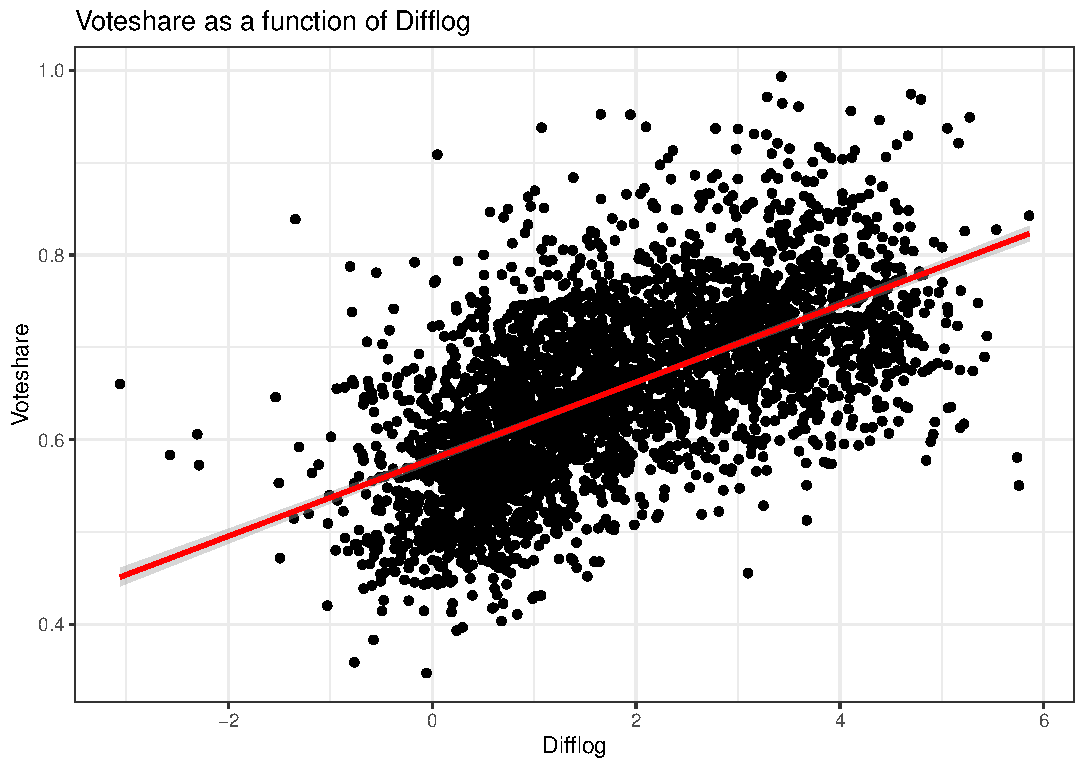
\includegraphics[width=.85\textwidth]{Q1graph.pdf}
		\end{figure}
		
		
		\item \textbf{Save the residuals of the model in a separate object.}
		\vspace{.25cm}
		
		\lstinputlisting[language=R, firstline=76, lastline=77]{PS03_CaitlinCooney_16322496.R}
		\vspace{.1cm}
		
		
		\vspace{.25cm}
		\item \textbf{Write the prediction equation.}
		
		\noindent The estimated regression line equation can be written as follows: 
		\newline 
		voteshare = 0.58 + 0.04*difflog
		
	\end{enumerate}
	
	\newpage
	
	\section*{Question 2}
	\noindent We are interested in knowing how the difference between incumbent and challenger's spending and the vote share of the presidential candidate of the incumbent's party are related.
	\vspace{.25cm}
	\begin{enumerate}
		\item \textbf{Run a regression where the outcome variable is \texttt{presvote} and the explanatory variable is \texttt{difflog}.}	\vspace{.25cm}
		
		\lstinputlisting[language=R, firstline=101, lastline=106]{PS03_CaitlinCooney_16322496.R}
		\vspace{.1cm}
		
		\begin{table}[!htbp] \centering 
			\caption{Difflog-Presvote Regression} 
			\label{} 
			\begin{tabular}{@{\extracolsep{5pt}}lc} 
				\\[-1.8ex]\hline 
				\hline \\[-1.8ex] 
				& \multicolumn{1}{c}{\textit{Dependent variable:}} \\ 
				\cline{2-2} 
				\\[-1.8ex] & presvote \\ 
				\hline \\[-1.8ex] 
				difflog & 0.024$^{***}$ \\ 
				& (0.001) \\ 
				& \\ 
				Constant & 0.508$^{***}$ \\ 
				& (0.003) \\ 
				& \\ 
				\hline \\[-1.8ex] 
				Observations & 3,193 \\ 
				R$^{2}$ & 0.088 \\ 
				Adjusted R$^{2}$ & 0.088 \\ 
				Residual Std. Error & 0.110 (df = 3191) \\ 
				F Statistic & 307.715$^{***}$ (df = 1; 3191) \\ 
				\hline 
				\hline \\[-1.8ex] 
				\textit{Note:}  & \multicolumn{1}{r}{$^{*}$p$<$0.1; $^{**}$p$<$0.05; $^{***}$p$<$0.01} \\ 
			\end{tabular} 
		\end{table} 
		
		
		
		\item \textbf{Make a scatterplot of the two variables and add the regression line. }	\vspace{.25cm}
		
		\lstinputlisting[language=R, firstline=110, lastline=116]{PS03_CaitlinCooney_16322496.R}
		\vspace{.1cm}
		
		\begin{figure}[!htbp]\centering
			\caption{\footnotesize Difflog-Presvote Regression}
			\label{fig:plot_5}
			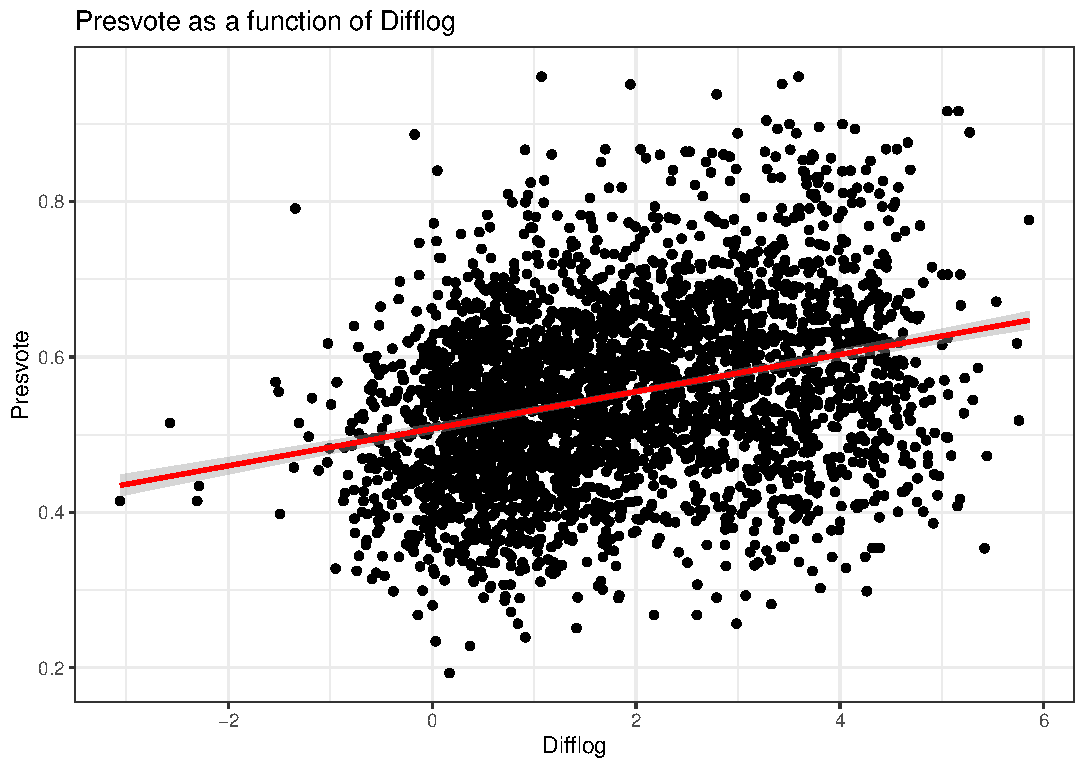
\includegraphics[width=.85\textwidth]{Q2graph.pdf}
		\end{figure}
		
		\item \textbf{Save the residuals of the model in a separate object.}	\vspace{.25cm}
		
		\lstinputlisting[language=R, firstline=121, lastline=122]{PS03_CaitlinCooney_16322496.R}
		\vspace{.25cm}
		
		\item \textbf{Write the prediction equation.}
		
		\noindent The estimated regression line equation can be written as follows: 
		\newline 
		presvote = 0.51 + 0.02*difflog 
		
	\end{enumerate}
	
	\newpage	
	\section*{Question 3}
	
	\noindent We are interested in knowing how the vote share of the presidential candidate of the incumbent's party is associated with the incumbent's electoral success.
	\vspace{.25cm}
	\begin{enumerate}
		\item \textbf{Run a regression where the outcome variable is \texttt{voteshare} and the explanatory variable is \texttt{presvote}.}
		\vspace{.25cm}
		
		\lstinputlisting[language=R, firstline=138, lastline=143]{PS03_CaitlinCooney_16322496.R}
		
		
		\begin{table}[!htbp] \centering 
			\caption{Presvote-Voteshare Regression} 
			\label{} 
			\begin{tabular}{@{\extracolsep{5pt}}lc} 
				\\[-1.8ex]\hline 
				\hline \\[-1.8ex] 
				& \multicolumn{1}{c}{\textit{Dependent variable:}} \\ 
				\cline{2-2} 
				\\[-1.8ex] & voteshare \\ 
				\hline \\[-1.8ex] 
				presvote & 0.388$^{***}$ \\ 
				& (0.013) \\ 
				& \\ 
				Constant & 0.441$^{***}$ \\ 
				& (0.008) \\ 
				& \\ 
				\hline \\[-1.8ex] 
				Observations & 3,193 \\ 
				R$^{2}$ & 0.206 \\ 
				Adjusted R$^{2}$ & 0.206 \\ 
				Residual Std. Error & 0.088 (df = 3191) \\ 
				F Statistic & 826.950$^{***}$ (df = 1; 3191) \\ 
				\hline 
				\hline \\[-1.8ex] 
				\textit{Note:}  & \multicolumn{1}{r}{$^{*}$p$<$0.1; $^{**}$p$<$0.05; $^{***}$p$<$0.01} \\ 
			\end{tabular} 
		\end{table} 
		
		
		\vspace{.1cm}
		\newpage
		\item \textbf{Make a scatterplot of the two variables and add the regression line. }
		\vspace{.25cm}
		
		\lstinputlisting[language=R, firstline=147, lastline=153]{PS03_CaitlinCooney_16322496.R}
		
		\begin{figure}[!htbp]\centering
			\caption{\footnotesize Presvote-Voteshare Regression}
			\label{fig:plot_5}
			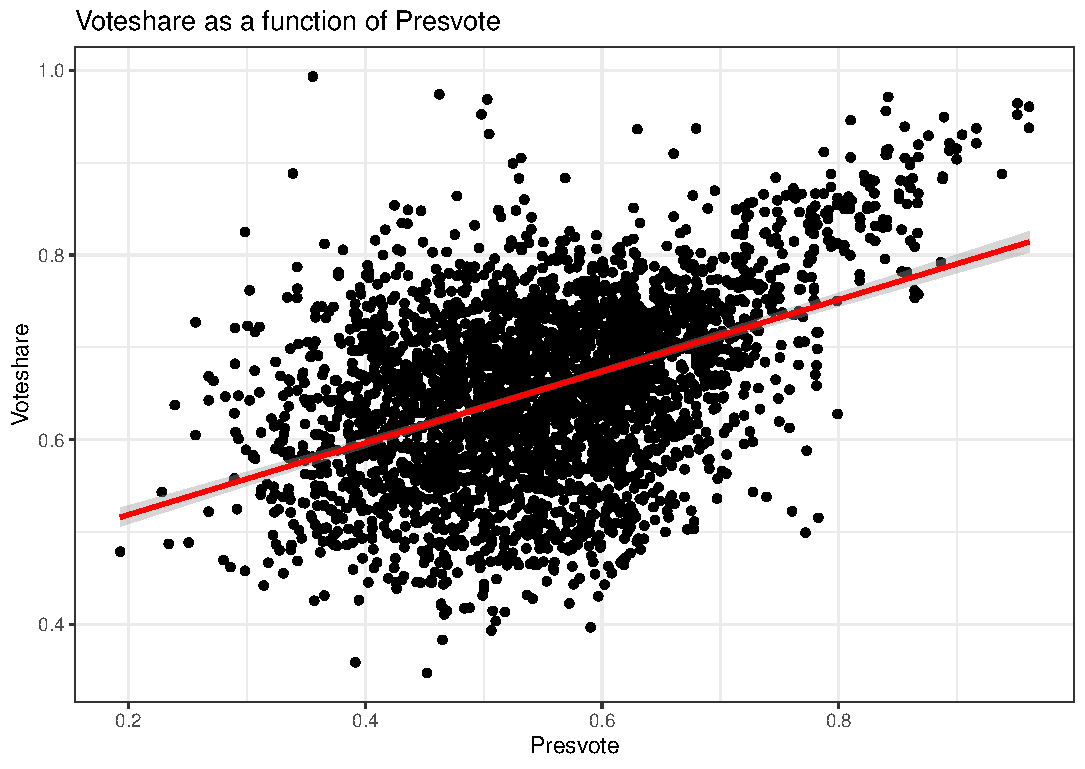
\includegraphics[width=.85\textwidth]{Q3graph.pdf}
		\end{figure}
		
		\noindent \item \textbf{Write the prediction equation.}
	\end{enumerate}
	
	\noindent \newline The estimated regression line equation can be written as follows: 
	\newline voteshare = 0.44 + 0.39*presvote
	
	
	\newpage	
	\section*{Question 4}
	\noindent The residuals from part (a) tell us how much of the variation in \texttt{voteshare} is $not$ explained by the difference in spending between incumbent and challenger. The residuals in part (b) tell us how much of the variation in \texttt{presvote} is $not$ explained by the difference in spending between incumbent and challenger in the district.
	\begin{enumerate}
		\item \textbf{Run a regression where the outcome variable is the residuals from Question 1 and the explanatory variable is the residuals from Question 2.}	\vspace{.25cm}
		
		\lstinputlisting[language=R, firstline=171, lastline=176]{PS03_CaitlinCooney_16322496.R}
		
		\begin{table}[!htbp] \centering 
			\caption{Q1 Residuals-Q2 Residuals Regression} 
			\label{} 
			\begin{tabular}{@{\extracolsep{5pt}}lc} 
				\\[-1.8ex]\hline 
				\hline \\[-1.8ex] 
				& \multicolumn{1}{c}{\textit{Dependent variable:}} \\ 
				\cline{2-2} 
				\\[-1.8ex] & Voteshare\_res \\ 
				\hline \\[-1.8ex] 
				Presvote\_res & 0.257$^{***}$ \\ 
				& (0.012) \\ 
				& \\ 
				Constant & $-$0.000 \\ 
				& (0.001) \\ 
				& \\ 
				\hline \\[-1.8ex] 
				Observations & 3,193 \\ 
				R$^{2}$ & 0.130 \\ 
				Adjusted R$^{2}$ & 0.130 \\ 
				Residual Std. Error & 0.073 (df = 3191) \\ 
				F Statistic & 476.975$^{***}$ (df = 1; 3191) \\ 
				\hline 
				\hline \\[-1.8ex] 
				\textit{Note:}  & \multicolumn{1}{r}{$^{*}$p$<$0.1; $^{**}$p$<$0.05; $^{***}$p$<$0.01} \\ 
			\end{tabular} 
		\end{table} 
		
		
		\newpage	\item \textbf{Make a scatterplot of the two residuals and add the regression line.} 	\vspace{.25cm}
		
		\lstinputlisting[language=R, firstline=180, lastline=186]{PS03_CaitlinCooney_16322496.R}
		
		\begin{figure}[!htbp]\centering
			\caption{\footnotesize Difflog-Voteshare Regression}
			\label{fig:plot_5}
			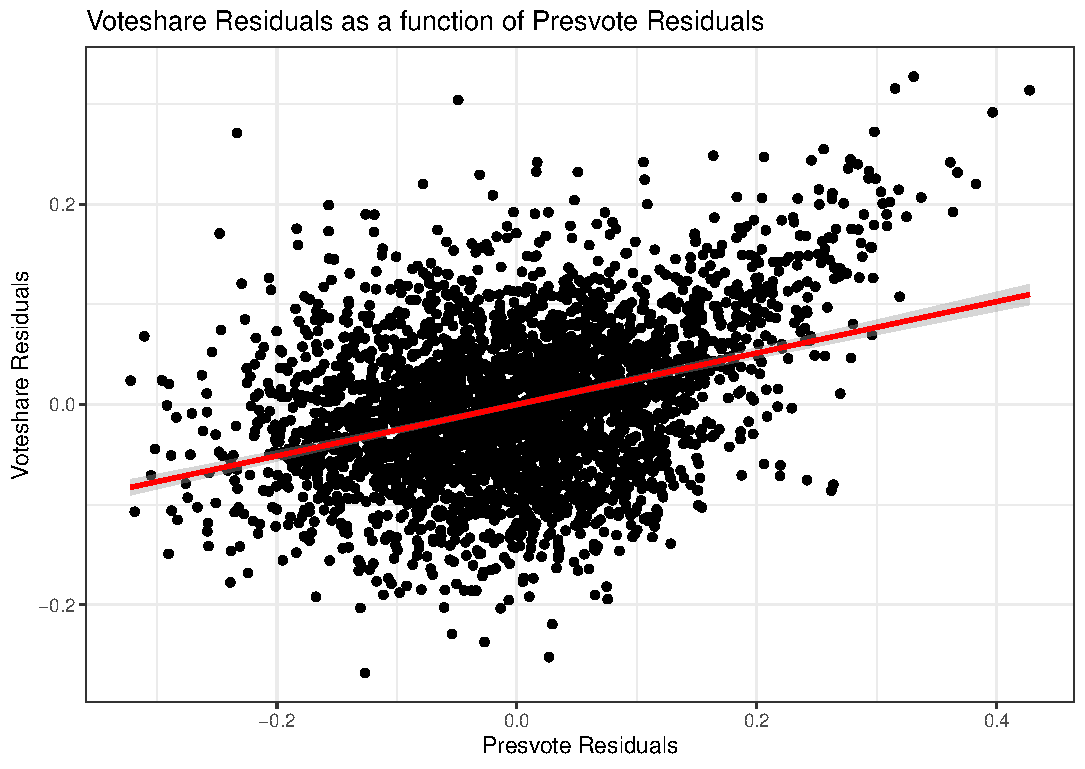
\includegraphics[width=.85\textwidth]{Q4graph.pdf}
		\end{figure}
		
		\item \textbf{Write the prediction equation.}
		\newline The estimated regression line equation can be written as follows: 
		\newline Q1Resid = -4.860e-18 + 2.569e-01*Q2Resid
	\end{enumerate}
	
	\newpage	
	
	\section*{Question 5}
	\noindent What if the incumbent's vote share is affected by both the president's popularity and the difference in spending between incumbent and challenger? 
	\begin{enumerate}
		\item \textbf{Run a regression where the outcome variable is the incumbent's \texttt{voteshare} and the explanatory variables are \texttt{difflog} and \texttt{presvote}.}	\vspace{.25cm}
		\lstinputlisting[language=R, firstline=201, lastline=206]{PS03_CaitlinCooney_16322496.R}
		
		\begin{table}[!htbp] \centering 
			\caption{Difflog and Presvote - Voteshare Regression} 
			\label{} 
			\begin{tabular}{@{\extracolsep{5pt}}lc} 
				\\[-1.8ex]\hline 
				\hline \\[-1.8ex] 
				& \multicolumn{1}{c}{\textit{Dependent variable:}} \\ 
				\cline{2-2} 
				\\[-1.8ex] & voteshare \\ 
				\hline \\[-1.8ex] 
				difflog & 0.036$^{***}$ \\ 
				& (0.001) \\ 
				& \\ 
				presvote & 0.257$^{***}$ \\ 
				& (0.012) \\ 
				& \\ 
				Constant & 0.449$^{***}$ \\ 
				& (0.006) \\ 
				& \\ 
				\hline \\[-1.8ex] 
				Observations & 3,193 \\ 
				R$^{2}$ & 0.450 \\ 
				Adjusted R$^{2}$ & 0.449 \\ 
				Residual Std. Error & 0.073 (df = 3190) \\ 
				F Statistic & 1,302.947$^{***}$ (df = 2; 3190) \\ 
				\hline 
				\hline \\[-1.8ex] 
				\textit{Note:}  & \multicolumn{1}{r}{$^{*}$p$<$0.1; $^{**}$p$<$0.05; $^{***}$p$<$0.01} \\ 
			\end{tabular} 
		\end{table} 
		
		
		\item \textbf{Write the prediction equation.}	\vspace{.25cm}
		
		\noindent The estimated regression line equation can be written as follows: 
		\newline voteshare = 0.45 + (0.04*difflog) + (0.26*presvote)
		
		\item \textbf{What is it in this output that is identical to the output in Question 4? Why do you think this is the case?}
		
		The Residual Std. Error	in the output for this question is identical to the 
		Residual Std. Error	in the output for Q4. 
		
		This is because running a regression of the residuals of voteshare $\sim$ difflog against 
		the residuals of presvote $\sim$ difflog as we do in Q4, tells us how much of the unexplained 
		variation in voteshare is influenced by presvote. 
		
		In Q5, we are essentially showing the same thing in a different way, by running 
		a regression of voteshare against difflog AND presvote, we can see how much of the unexplained 
		variance in voteshare $\sim$ difflog is explained by presvote,and this means that the Residual Std. Error will be the same. 
		
	\end{enumerate}
	
	
	
	
\end{document}
